\section{Auswertung}
\label{sec:Auswertung}

In \ref{tab:Tabelle1}. \ref{tab:Tabelle2} und \ref{tab:Tabelle3} sind die Werte für die gemessnen Sink- und Steigzeiten der 10 Öltröpfchen enthalten.

\begin{table}[http]
  \centering
  \caption{In dieser Tabelle ist die gemessene Sink- und Steigzeit von den ersten vier Öltröpchen eingetragen.}
  \label{tab:Tabelle1}
  \sisetup{table-format=1.1, per-mode=reciprocal}
  \begin{minipage}[t]{0.2\linewidth}
    \begin{tblr}[t]{
      colspec = {S[table-format=1.2] S[table-format=1.2] },
      row{1} = {guard, mode=math},
    }
    \toprule
    t_{sink} \mathbin{/} \unit{\second} & t_{steig} \mathbin{/} \unit{\second}  \\
    \midrule
    1.61  &  1.48 \\
    1.87  &  1.40 \\
    1.13  &  1.57 \\
    1.35  &  1.36 \\
    1.43  &  1.54 \\
    1.15  &  1.38 \\
    1.55  &  1.45 \\

    \bottomrule
  \end{tblr}
\end{minipage}
\hfill
\begin{minipage}[t]{0.2\linewidth}
    \begin{tblr}[t]{
      colspec = {S[table-format=1.2] S[table-format=1.2] },
      row{1} = {guard, mode=math},
    }
    \toprule
    t_{sink} \mathbin{/} \unit{\second} & t_{steig} \mathbin{/} \unit{\second}  \\
    \midrule
    2.28  &  2.37 \\
    2.43  &  2.41 \\
    2.21  &  2.40 \\
    2.65  &  2.06 \\
    2.44  &  2.73 \\
    \bottomrule
  \end{tblr}
\end{minipage}
\hfill
\begin{minipage}[t]{0.2\linewidth}
  \begin{tblr}[t]{
    colspec = {S[table-format=1.2] S[table-format=1.2] },
    row{1} = {guard, mode=math},
  }
  \toprule
  t_{sink} \mathbin{/} \unit{\second} & t_{steig} \mathbin{/} \unit{\second}  \\
  \midrule
  2.97  &  2.70 \\
  2.50  &  2.93 \\
  2.42  &  2.66 \\
  2.63  &  2.95 \\
  2.58  &  2.79 \\

  \bottomrule
\end{tblr}
\end{minipage}
\hfill
\begin{minipage}[t]{0.2\linewidth}
    \begin{tblr}[t]{
      colspec = {S[table-format=1.2] S[table-format=1.2] },
      row{1} = {guard, mode=math},
    }
    \toprule
    t_{sink} \mathbin{/} \unit{\second} & t_{steig} \mathbin{/} \unit{\second}  \\
    \midrule
    2.18  &  3.11 \\
    2.70  &  3.03 \\
    3.21  &  2.72 \\
    2.55  &  3.10 \\
    2.44  &  2.89 \\
    \bottomrule
  \end{tblr}
\end{minipage}
\end{table}

\begin{table}[http]
  \centering
  \caption{Hier ist die Sink- und Steigzeit von den Öltröpchen 5 bis 7 eingetragen.}
  \label{tab:Tabelle2}
  \sisetup{table-format=1.1, per-mode=reciprocal}
  \begin{minipage}[t]{0.3\linewidth}
    \begin{tblr}[t]{
      colspec = {S[table-format=1.2] S[table-format=1.2] },
      row{1} = {guard, mode=math},
    }
    \toprule
    t_{sink} \mathbin{/} \unit{\second} & t_{steig} \mathbin{/} \unit{\second}  \\
    \midrule
    3.59  &  4.64 \\
    3.62  &  4.93 \\
    3.74  &  4.61 \\
    3.73  &  4.96 \\
    3.88  &  4.63 \\

    \bottomrule
  \end{tblr}
\end{minipage}
\hfill
\begin{minipage}[t]{0.3\linewidth}
    \begin{tblr}[t]{
      colspec = {S[table-format=1.2] S[table-format=1.2] },
      row{1} = {guard, mode=math},
    }
    \toprule
    t_{sink} \mathbin{/} \unit{\second} & t_{steig} \mathbin{/} \unit{\second}  \\
    \midrule
    2.26  &  2.98 \\
    2.45  &  3.31 \\
    2.34  &  3.16 \\
    2.39  &  2.83 \\
    2.40  &  3.55 \\
    \bottomrule
  \end{tblr}
\end{minipage}
\hfill
\begin{minipage}[t]{0.3\linewidth}
  \begin{tblr}[t]{
    colspec = {S[table-format=1.2] S[table-format=1.2] },
    row{1} = {guard, mode=math},
  }
  \toprule
  t_{sink} \mathbin{/} \unit{\second} & t_{steig} \mathbin{/} \unit{\second}  \\
  \midrule
  4.73  &  4.98 \\
  4.91  &  4.86 \\
  4.56  &  5.69 \\
  4.39  &  6.72 \\
  4.82  &  5.38 \\

  \bottomrule
\end{tblr}
\end{minipage}
\end{table}


\begin{table}[http]
  \centering
  \caption{In der Tabelle ist die gemessene Sink- und Steigzeit von den letzten drei Öltröpchen aufgeführt.}
  \label{tab:Tabelle3}
  \sisetup{table-format=1.1, per-mode=reciprocal}
  \begin{minipage}[t]{0.3\linewidth}
    \begin{tblr}[t]{
      colspec = {S[table-format=1.2] S[table-format=1.2] },
      row{1} = {guard, mode=math},
    }
    \toprule
    t_{sink} \mathbin{/} \unit{\second} & t_{steig} \mathbin{/} \unit{\second}  \\
    \midrule
    4.35  &  8.69 \\
    5.90  &  7.87 \\
    5.99  &  8.48 \\
    5.62  &  7.72 \\
    5.89  &  6.64 \\

    \bottomrule
  \end{tblr}
\end{minipage}
\hfill
\begin{minipage}[t]{0.3\linewidth}
    \begin{tblr}[t]{
      colspec = {S[table-format=1.2] S[table-format=1.2] },
      row{1} = {guard, mode=math},
    }
    \toprule
    t_{sink} \mathbin{/} \unit{\second} & t_{steig} \mathbin{/} \unit{\second}  \\
    \midrule
    3.19  &  4.55 \\
    3.86  &  4.48 \\
    3.63  &  4.31 \\
    3.71  &  4.39 \\
    3.96  &  4.65 \\
    \bottomrule
  \end{tblr}
\end{minipage}
\hfill
\begin{minipage}[t]{0.3\linewidth}
  \begin{tblr}[t]{
    colspec = {S[table-format=1.2] S[table-format=2.2] },
    row{1} = {guard, mode=math},
  }
  \toprule
  t_{sink} \mathbin{/} \unit{\second} & t_{steig} \mathbin{/} \unit{\second}  \\
  \midrule
  6.11  &   8.74 \\
  7.73  &   9.92 \\
  6.84  &   9.79 \\
  7.26  &   9.99 \\
  6.44  &  11.22 \\

  \bottomrule
\end{tblr}
\end{minipage}
\end{table}

Mit der Formel 
\begin{equation*}
  \bar{t}=\frac{1}{n} \sum_{i=1}^n t_i
\end{equation*}
wird der Mittelwert der Sink- und Steigzeiten ausgerechnet und in \ref{tab:Mittelwerte} eingetragen.
Dazu werden auch die Standardabweichungen, berechnet mit 
\begin{equation*}  
  s=\sqrt{\frac{1}{N-1} \sum_{i=1}^N (t_i-\bar{t})^2}
\end{equation*}
berechnet.

\begin{table}[H]
  \centering
  \caption{Aufgeführt sind die Mittelwerte der Sinkzeiten, sowie die entsprechenden Mittelwerte der Steigzeiten mit deren Fehlern.}
  \label{tab:Mittelwerte}
  \sisetup{table-format=1.1, per-mode=reciprocal}
    \begin{tblr}[t]{
      colspec = {S[table-format=2.0] S[table-format=1.3] S[table-format=1.3] S[table-format=1.3] S[table-format=1.3] },
      row{1} = {guard, mode=math},
      vline{3}={2}{-}{text=\clap{$\pm$}},
      vline{5}={2}{-}{text=\clap{$\pm$}},
    }
    \toprule
    N& t_{sink} \mathbin{/} \unit{\second} & & t_{steig} \mathbin{/} \unit{\second} &  \\
    \midrule
    1& 1.441 & 0.243 &   1.454  & 0.074 \\
    2& 2.402 & 0.152 &   2.394  & 0.212\\
    3& 2.620 & 0.189 &   2.806  & 0.117\\
    4& 2.616 & 0.342 &   2.970  & 0.148\\
    5& 3.712 & 0.103 &   4.754  & 0.156\\
    6& 2.368 & 0.064 &   3.166  & 0.251\\
    7& 4.682 & 0.186 &   5.526  & 0.665\\
    8& 5.550 & 0.612 &   7.880  & 0.718\\
    9& 3.670 & 0.266 &   4.476  & 0.119\\
   10& 6.876 & 0.575 &   9.932  & 0.788\\
    \bottomrule
  \end{tblr}
\end{table}

Da $d=\qty{7.6250(0.0051)}{\milli\meter}$ bekannt ist, kann die Geschwindigkeit $v$ der einzelnen Öltröpfchen mit 
\begin{equation}
  v=\frac{s}{t}
\end{equation}
berechnet werden. 
Diese wurden in die Tabelle \ref{tab:Geschwindigkeiten} eingetragen.


\begin{table}[H]
  \centering
  \caption{Hier sind die Geschwindigkeiten der Öltropfchen eingetragen.}
  \label{tab:Geschwindigkeiten}
  \sisetup{table-format=1.1, per-mode=reciprocal}
    \begin{tblr}[t]{
      colspec = {S[table-format=2.0] S[table-format=1.3] S[table-format=1.3] S[table-format=1.3] S[table-format=1.3] },
      row{1} = {guard, mode=math},
      vline{3}={2}{-}{text=\clap{$\pm$}},
      vline{5}={2}{-}{text=\clap{$\pm$}},
    }
    \toprule
    N &v_{sink} \mathbin{/} \unit{\meter\per\milli\second} & & v_{steig} \mathbin{/}  \unit{\meter\per\milli\second}&  \\
    \midrule
    1  & 0.360 & 0.060 & 0.345 & 0.017 \\
    2  & 0.209 & 0.013 & 0.211 & 0.019 \\ 
    3  & 0.192 & 0.013 & 0.179 & 0.007 \\ 
    4  & 0.194 & 0.024 & 0.169 & 0.009 \\ 
    5  & 0.135 & 0.004 & 0.105 & 0.003 \\
    6  & 0.211 & 0.006 & 0.159 & 0.013 \\ 
    7  & 0.107 & 0.004 & 0.092 & 0.010 \\
    8  & 0.091 & 0.012 & 0.064 & 0.006 \\ 
    9  & 0.137 & 0.011 & 0.112 & 0.003 \\ 
   10  & 0.073 & 0.006 & 0.051 & 0.004 \\
    \bottomrule
  \end{tblr}
\end{table}

Mit der Formel \ref{eqn:Radius} wurden dann die Radien $r$ der einzelnen Öltröpfchen berechnet und in die Tabelle \ref{tab:Radien} eingetragen.


\begin{table}[H]
  \centering
  \caption{In dieser Tabelle sind die berechneten Radien $r$ der Tröpfchen aufgeführt.}
  \label{tab:Radien}
  \sisetup{table-format=1.1, per-mode=reciprocal}
    \begin{tblr}[t]{
      colspec = {S[table-format=2.0] S[table-format=1.3] S[table-format=1.3] },
      row{1} = {guard, mode=math},
      vline{3}={2}{-}{text=\clap{$\pm$}},
    }
    \toprule
    N &r \mathbin{/} \unit{\micro\meter} &  \\
    \midrule
    1&0.200 & 0.600 \\
    3&0.250 & 0.140 \\
    4&0.350 & 0.180 \\ 
    5&0.374 & 0.032 \\ 
    6&0.500 & 0.070 \\ 
    7&0.270 & 0.100 \\ 
    8&0.360 & 0.090 \\ 
    9&0.350 & 0.080 \\ 
   10&0.330 & 0.050 \\
    \bottomrule
  \end{tblr}
\end{table}


Mit \ref{eqn:Ladung} wird dann die Ladung der Öltropfchen berechnet.
Diese wird in für alle der Tabelle \ref{tab:Ladungen} gesammelt.


\begin{table}[H]
  \centering
  \caption{Hier werden die Ladungen $q$ der Tröpfchen eingetragen.}
  \label{tab:Ladungen}
  \sisetup{table-format=1.1, per-mode=reciprocal}
    \begin{tblr}[t]{
      colspec = {S[table-format=2.0] S[table-format=1.3] S[table-format=1.3] },
      row{1} = {guard, mode=math},
      vline{3} = {2}{-}{text=\clap{$\pm$}},
    }
    \toprule
    N &q \mathbin{/} \unit{\coulomb} \cdot 10^{-19} &  &\\
    \midrule
    2&3.236 & 2.561 \\
    4&4.884 & 3.428 \\
    5&3.547 & 0.396 \\
    6&7.800 & 1.079 \\
    7&1.909 & 0.860 \\
    8&2.190 & 0.809 \\
    9&3.326 & 1.064 \\
   10&1.541 & 0.369 \\
    \bottomrule
  \end{tblr}
\end{table}

Daraufhin werden die Werte gegen die Nummer des Öltröpfchens in Abbildung \ref{fig:Ladung} aufgetragen und Stufen hinzugefügt, welche Vielfaches von dem niedrigsten Wert, also $q_10=\qty{1.541( 0.369)e-19}{\coulomb}$ darstellen.
Die Höhe von den Balken ist  $h=\qty{1e-19}{\coulomb}$.

\begin{figure}
  \centering
  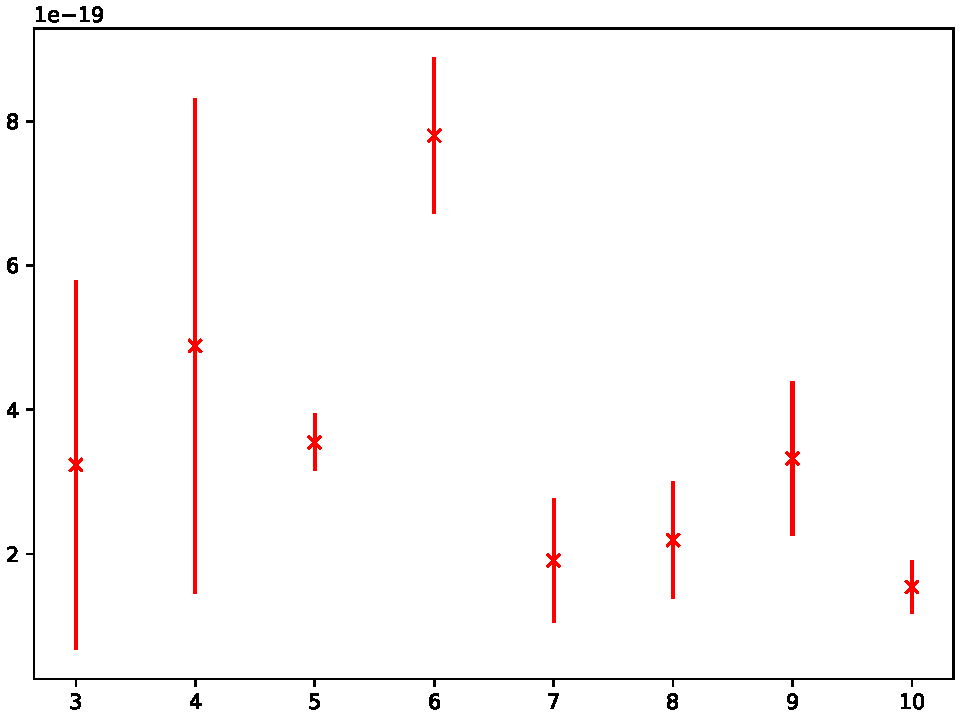
\includegraphics[width=\textwidth]{build/Daten.pdf}
  \caption{Hier ist die Ladung der Tröpfchen in Abhängigkeit zu dessen Nummer geplottet.
  Dazu wurden Balken eingefügt, dessen y-Wert ein Vielfaches von $q_10$ ist.}
  \label{fig:Ladung}
\end{figure}